\documentclass[10pt, a4paper]{article}

\usepackage[utf8]{inputenc}
\usepackage[english, spanish]{babel}
\usepackage[left=25mm, right=25mm, top=35mm, bottom=30mm, headheight=35mm]{geometry}
\usepackage{graphicx}
\usepackage{float}
\usepackage{xcolor}
\usepackage{fancyhdr}
\usepackage{hyperref}
\usepackage{setspace}
\usepackage{indentfirst}

% Syntax customization with minted package
\usepackage{minted}
\usemintedstyle{nord-darker}
\usemintedstyle[zsh]{gruvbox-light}
\setminted{
  breaklines,
  linenos,
  frame=lines,
  fontsize=\normalsize
}
\newcommand{\mpy}[1]{\mintinline[style=gruvbox-light]{python}{#1}}

% Define background color
\definecolor{background}{HTML}{2E3440}

% Variables
\newcommand{\university}{Universidad Nacional de San Agustín de Arequipa}
\newcommand{\faculty}{Facultad de Ingeniería de Producción y Servicios}
\newcommand{\program}{Escuela Profesional de Ingeniería de Sistemas}
\newcommand{\semester}{2024 - A}
\newcommand{\course}{img/web_programming.png}
\newcommand{\topic}{img/relationship_pdf_emails.png}
\newcommand{\professor}{Carlo Jose Luis Corrales Delgado}
\newcommand{\student}{Jorge Luis Mamani Huarsaya}
\newcommand{\email}{https://mail.google.com/mail/u/0/?fs=1&tf=cm&source=mailto&to=jmamanihuars@unsa.edu.pe}
\newcommand{\github}{https://github.com/jorghee/django-projects}
\newcommand{\mydate}{15 de junio, 2024}

% Just parts and chapters numbered
\setcounter{secnumdepth}{0}

% Head and foot customization
\pagestyle{fancy}
\lhead{\raisebox{-0.2\height}{
\includegraphics[width=4cm]{img/logo_unsa.png}}}
\chead{\fontsize{8}{8}\selectfont \university \\ \faculty \\ \textbf{\program}}
\rhead{\raisebox{-0.2\height}{
\includegraphics[width=3.5cm]{img/logo_episunsa.png}}}
\lfoot{Estudiante \student}
\cfoot{}
\rfoot{Pág. \thepage}

\begin{document}

\begin{titlepage}
	\centering
	\includegraphics[width=15cm]{\course} \par
  \vfill \vfill
	\includegraphics[width=15cm]{\topic}\par
  \vfill \vfill
  {\textbf{Profesor(a):} \par}
	\professor \vfill
  {\textbf{Estudiante:} \par}
	\student \vfill
  {\textbf{Email:} \par}
  \href{\email}{jmamanihuars@unsa.edu.pe} \vfill
  {\textbf{Repositorio GitHub:} \par}
  \href{\github}{\github} \vfill
	{\large \mydate \par}
\end{titlepage}

\section{Tipos de relaciones en la base de datos con Django}
El sistema de gestión de base de datos que se está utilizando en esta oportunidad es PostgreSQL, por lo tanto empezamos creando un un proyecto \mpy{django_relationships} Django y dentro de este proyecto creamos la aplicación \mpy{relationships}. Antes de enfocarnos en la creación de modelos Django, nos dirigimos al archivo \mpy{settings.py} del proyecto donde modificamos la base de datos por defecto.

\begin{minted}[bgcolor=background]{python}
DATABASES = {
  'default': {
    'ENGINE': 'django.db.backends.postgresql',
    'NAME': env('DB_NAME'),
    'USER': env('DB_USER'),
    'PASSWORD': env('DB_PASSWORD'),
    'HOST': env('DB_HOST'),
    'PORT': env('DB_PORT'),
  }
}
\end{minted}

\subsection{Relación uno a muchos}
Hemos creado 2 modelos en Django: Language y Framework donde podemos apreciar esta relación, pues un Language puede tener varios Frameworks, sin embargo un Framework solo puede tener un Language. Para proporcionar esta caracteristica, Django nos permite usar el método \mpy{ForeignKey} donde indica que esta variable es una clave foránea.

\begin{minted}[bgcolor=background]{python}
class Language(models.Model):
  name = models.CharField(max_length=10)

  def __str__(self):
    return self.name

class Framework(models.Model):
  name = models.CharField(max_length=10)
  language = models.ForeignKey(Language, on_delete=models.CASCADE)

  def __str__(self):
    return self.name
\end{minted}

Para realizar las pruebas usando la shell de Python, necesitamos informarle a Django de la existencia de la aplicación \mpy{relationships} en el archivo de configuracion \mpy{settings.py} y luego crear y realizar las migraciones en nuestra base de datos, en este caso estamos usando en sistema de gestion de base de datos PostgreSQL.

\begin{minted}[bgcolor=background]{python}
INSTALLED_APPS = [
    'relationships',
\end{minted}

Ahora si podemos realizar las pruebas usando la shell de python, por ejemplo vamos a crear objetos de los modelos Language y Framework.

\begin{figure}[H]
  \centering
  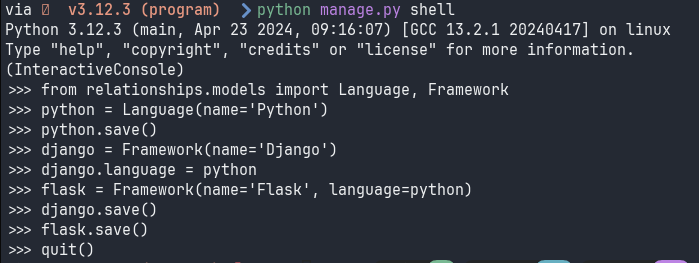
\includegraphics[width=0.8\textwidth]{img/1_create_lan_fra.png}
  \caption{Filas en la base de datos}
\end{figure}

La funcionalidad de Django se ve en las siguientes operaciones como son filtrar de acuerdo a un campo especifico. Primeramente veremos en nuestra base de datos que el campo \mpy{language} en el modelo Framework, se creará automaticamente como \mpy{language_id} en la tabla  Framework en la base de datos. Este campo almacena el \mpy{id} del Language relacionado.
\singlespacing

\begin{figure}[H]
  \centering
  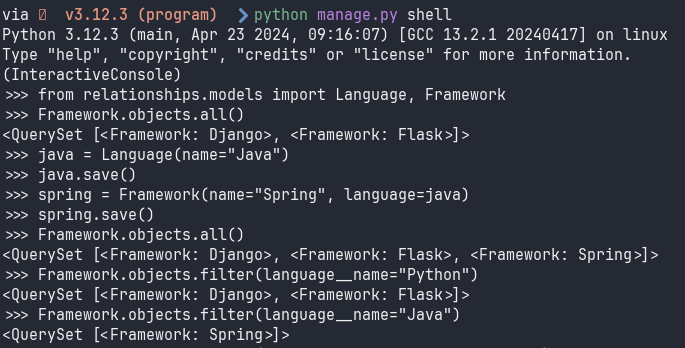
\includegraphics[width=0.8\textwidth]{img/2_filter.png}
  \caption{Uso del doble guión bajo}
\end{figure}

Como vemos y somos observadores, nos preguntaremos a qué referencia \mpy{language__name}. Esta es una funcionalidad de Django para seguir las relaciones entre los modelos y realizar consultas a través de esas relaciones.

\begin{itemize}
  \item \textbf{language:} Este es el nombre del campo de clave foránea en el modelo Framework que hace referencia al modelo Language. Este campo establece una relación entre los modelos Framework y Language.

  \item \textbf{\_\_name:} La notación de doble guion bajo \mpy{__} indica a Django que queremos realizar una consulta a través de la relación establecida por el campo language. El campo language es una instancia del modelo Language, y queremos acceder a su campo name.
\end{itemize}

Ahora nos surge otra duda, si decimos que \mpy{language} es el campo en Django de clave foránea que referencia a una instancia Language, entonces, \textbf{por qué se puede realizar la siguiente consulta si en Language no hay ningún campo foráneo que referencia a Framework?}

\begin{minted}[bgcolor=background]{python}
Language.objects.filter(framework__name="Spring")
\end{minted}

Lo que pasa es que en Django, cuando definimos una relación de clave foránea en un modelo automáticamente crea una relación inversa en el modelo relacionado. Esto nos permite realizar consultas desde ambos lados de la relación.

\subsection{Relacion muchos a muchos}
Para mostrar esta relación, creamos las clases \mpy{Movie} y \mpy{Character} como modelos en Django, que establecerá la relacion entre películas y personajes. Podemos intuir la necesidad de esta relación para este caso ya que una película puede tener varios personajes y viceversa, un personaje puede participara en varias películas..

\begin{minted}[bgcolor=background]{python}
class Movie(models.Model):
  name = models.CharField(max_length=100)

  def __str__(self):
    return self.name

class Character(models.Model):
  name = models.CharField(max_length=100)
  movies = models.ManyToManyField(Movie)

  def __str__(self):
    return self.name
\end{minted}

Ahora podemos realizar las siguiente operaciones para poder observar cómo es que Django maneja este tipo de relación yqué es lo que hace en la base datos.

\begin{figure}[H]
  \centering
  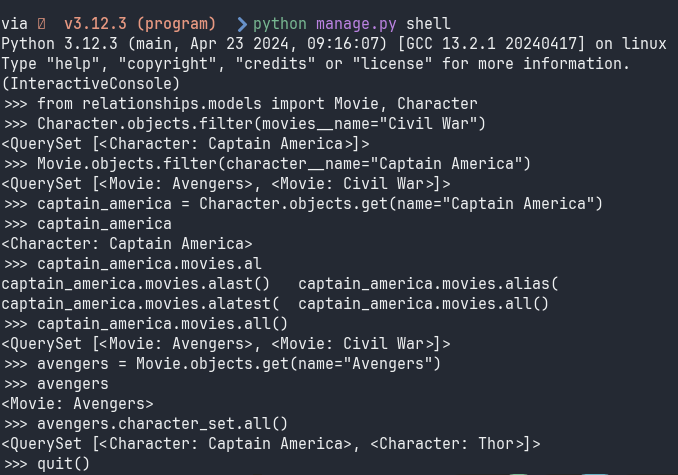
\includegraphics[width=0.8\textwidth]{img/3_many_to_many.png}
  \caption{Relación muchos a muchos}
\end{figure}

En la base de datos, Django maneja las relaciones de muchos a muchos utilizando una tabla intermedia que vincula las claves primarias de ambos modelos relacionados. Por ejemplo, para las relaciones anteriores, tenemos una tabla intermedia que se ve asi:

\begin{figure}[H]
  \centering
  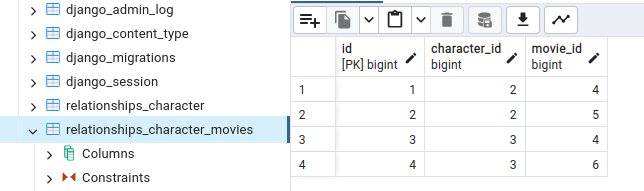
\includegraphics[width=0.8\textwidth]{img/4_intermediate_table.png}
  \caption{Tabla intermedia generada automáticamente}
\end{figure}

\section{Generación de PDFs con Django}
Para evidenciar esta funcionalidad, solo se ha creado un nuevo proyecto en el cual directamente implementamos la lógica para generar el pdf. Sin embargo tuvimos que hacer algunas configuraciones importantes en el archivo \mpy{settings.py}, como es habilitar el directorio \mpy{templates} para crear plantillas y tambien modificar el idioma y la hora de la zona.

\begin{minted}[bgcolor=background]{python}
TEMPLATES = [
    {
        'BACKEND': 'django.template.backends.django.DjangoTemplates',
        'DIRS': [os.path.join(BASE_DIR, 'templates')],
\end{minted}

\begin{minted}[bgcolor=background]{python}
LANGUAGE_CODE = 'es'
TIME_ZONE = 'America/Lima'
\end{minted}

Ahora, se ha creado el archivo \mpy{renderers.py} que se encarga de parsear el HTML a PDF, para esta funcionalidad se ha tenido que instalar el paquete \mpy{xhtml2pdf} de Python.

\begin{minted}[bgcolor=background]{python}
from io import BytesIO
from django.http import HttpResponse
from django.template.loader import get_template

from xhtml2pdf import pisa

def render_to_pdf(template_src, context_dict={}):
  template = get_template(template_src)
  html  = template.render(context_dict)
  result = BytesIO()
  pdf = pisa.pisaDocument(BytesIO(html.encode("ISO-8859-1")), result)
  if pdf.err:
    return HttpResponse("Invalid PDF", status_code=400, content_type='text/plain')
  return HttpResponse(result.getvalue(), content_type='application/pdf')
\end{minted}

Despues de crear este archivo, vamos a crear un vista que se encague de manejar la solicitud del cliente.

\begin{minted}[bgcolor=background]{python}
from django.http import Http404
import datetime
from . import renderers

def pdf_view(request, *args, **kwargs):
  data = {
    'pdf_title': "Factura Rovistar",
    'today': datetime.date.today(), 
    'amount': 39.99,
    'customer_name': 'Jorge Luis Mamani Huarsaya',
    'invoice_number': 1233434,
  }
  return renderers.render_to_pdf('pdf/invoice.html', data)
\end{minted}

Finalmente realizamos el direccionamiento modificando el archivo \mpy{urls.py}

\begin{minted}[bgcolor=background]{python}
from django.contrib import admin
from django.urls import path

from .views import pdf_view

urlpatterns = [
    path('', pdf_view, name="pdf_view"),
    path('admin/', admin.site.urls),
]
\end{minted}

Lanzamos el servidor local y probamos la funcionalidad. Nos daremos cuenta que accediendo desde la URL de nuestro navegador, se verá el pdf generado.

\section{Envio de correos electronicos con Django}
Comenzamos realizando las configuraciones en el archivo \mpy{settings.py} para que se pueda usar el servicio de envio de correos electrónicos.

\begin{minted}[bgcolor=background]{python}
EMAIL_BACKEND = 'django.core.mail.backends.smtp.EmailBackend'
EMAIL_HOST = 'smtp.gmail.com'
EMAIL_PORT = 587
EMAIL_HOST_USER = env('EMAIL_USER')
EMAIL_HOST_PASSWORD = env('EMAIL_PASSWORD')
EMAIL_USE_TLS = True
EMAIL_USE_SSL = False
\end{minted}

Ahora, creamos una aplicación denominada \mpy{send} y creamos una vista que se encarga de la lógica de manejar la solicitud del cliente. En este caso solo enviaremos directamente el email cuando se acceda a este sitio web.

\begin{minted}[bgcolor=background]{python}
from django.shortcuts import render
from django.core.mail import send_mail
from django.conf import settings

# Create your views here.
def index(request):

  subject = "Hello, is Jorghee"
  message = "I am programmer, I like the apples and penguins"
  email_from = settings.EMAIL_HOST_USER
  recipient_list = ['mamannihuarsaya4b@gmail.com']

  report = "Correo enviado exitosamente"
  try:
    send_mail(subject, message, email_from, recipient_list, fail_silently=False)
  except Exception as e:
    report = "Error al enviar el correo"
    print(e)

  return render(request, 'send/index.html', { "report":report })
\end{minted}

Como vemos, estamos renderizando una plantilla. Esta plantilla nos indicará si se realizo correctamente el envio del correo electrónico. Luego de hacer estas modificaciones, tenemos que direccionar las solicitudes modificando el archivo \mpy{urls.py} del proyecto y creando el archivo \mpy{urls.py} de la aplicación.
\end{document}
